\begin{figure}[H]
    \centering
    \definecolor{groundgreen}{RGB}{90,145,75}
    \definecolor{atmosblue}{RGB}{130,195,230}
    \definecolor{warmorange}{RGB}{245,175,85}
    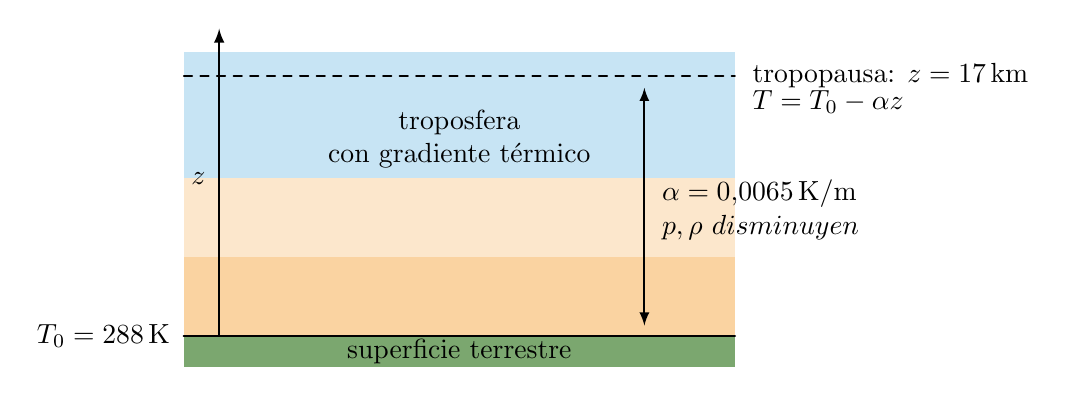
\begin{tikzpicture}[x=1cm,y=1cm,line cap=round,line join=round]
        % Columna atmosférica
        \fill[groundgreen!80] (1.0,0.35) rectangle (8.0,0.75);
        \fill[warmorange!55] (1.0,0.75) rectangle (8.0,1.75);
        \fill[warmorange!30] (1.0,1.75) rectangle (8.0,2.75);
        \fill[atmosblue!45] (1.0,2.75) rectangle (8.0,4.35);
        \draw[line width=0.9pt] (1.0,0.75) -- (8.0,0.75);

        % Eje vertical y tropopausa
        \draw[-latex,line width=0.75pt] (1.45,0.75) -- (1.45,4.65);
        \node[left] at (1.40,2.75) {$z$};
        \draw[dashed,line width=0.7pt] (1.0,4.05) -- (8.0,4.05);
        \node[right] at (8.10,4.05) {tropopausa: $z=17\,\mathrm{km}$};

        % Temperaturas y gradiente
        \node[left] at (0.95,0.75) {$T_0=288\,\mathrm{K}$};
        \node[right] at (8.10,3.72) {$T=T_0-\alpha z$};
        \draw[latex-latex,line width=0.65pt] (6.85,0.88) -- (6.85,3.90);
        \node[right,align=left] at (6.95,2.35)
            {$\alpha=0{,}0065\,\mathrm{K/m}$\\
             $p,\rho\ \text{disminuyen}$};

        \node at (4.50,0.55) {superficie terrestre};
        \node[align=center] at (4.50,3.25)
            {troposfera\\con gradiente térmico};
    \end{tikzpicture}
    \caption{Modelo de atmósfera con temperatura lineal usado en el problema 3.}
\end{figure}